\scalebox{0.8}{ % Adjust scale if needed
	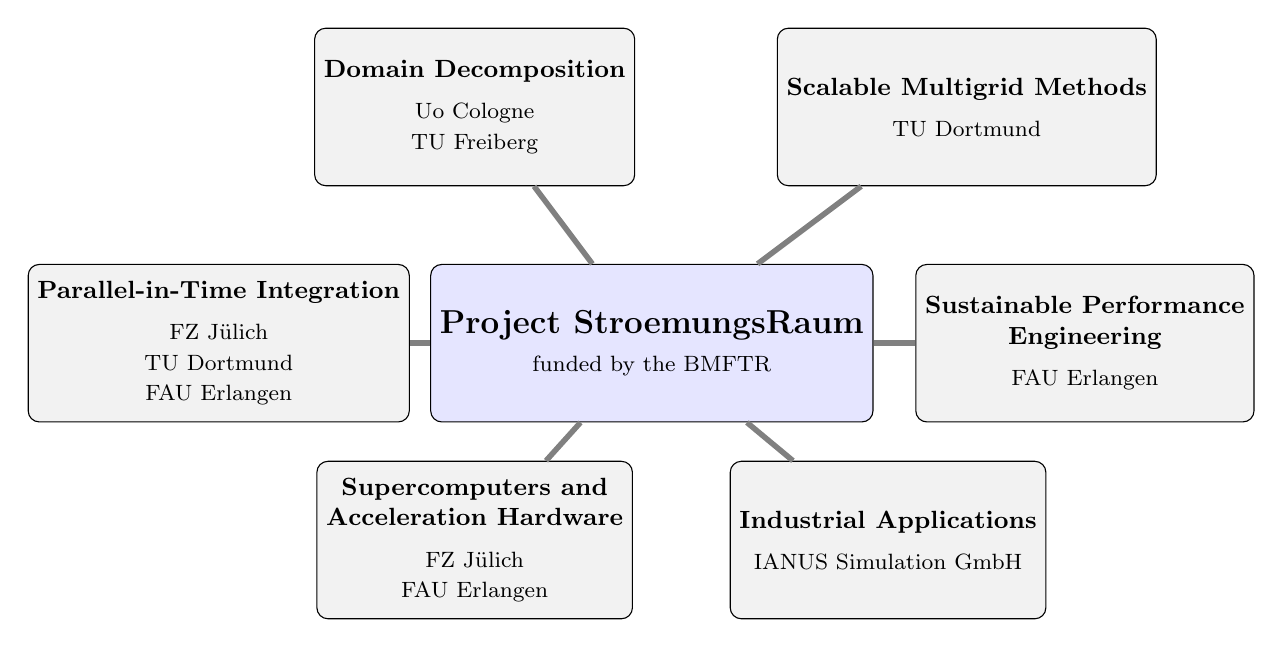
\begin{tikzpicture}[
			% Removed "mindmap" as it applies specific styling that's hard to override
			every node/.style={
					rectangle,
					rounded corners,
					minimum width=2cm,
					minimum height=2cm,
					align=center,
					font=\small,
					text=black,
					draw=black,
					fill=gray!10
				},
			root concept/.style={
					fill=blue!10,
					font=\bfseries\large,
					text=black,
					minimum width=3cm
				},
			% Custom edge style
			conn/.style={
					draw=black!50,
					line width=2pt,
					solid
				},
		]
		\begin{scope}[shift={(-5, 3)}]
			\node[root concept] (root) {Project StroemungsRaum\\{\normalfont\footnotesize funded by the BMFTR}};

			% Create child nodes with explicit positioning and manual edges
			\node[xshift=5.5cm, yshift=0cm] (n1) {\bf{Sustainable Performance}\\\bf{Engineering}\\[1ex]\footnotesize FAU Erlangen};
			\node[xshift=4cm, yshift=3cm] (n2) {\bf{Scalable Multigrid Methods}\\[1ex] \footnotesize TU Dortmund};
			\node[xshift=-2.25cm, yshift=3cm] (n3) {\bf{Domain Decomposition}\\[1ex]\footnotesize \alert{Uo Cologne}\\ \footnotesize TU Freiberg};
			\node[xshift=-5.5cm, yshift=0cm] (n4) {\bf{Parallel-in-Time Integration}\\[1ex] \footnotesize FZ Jülich\\ \footnotesize TU Dortmund\\ \footnotesize FAU Erlangen};
			\node[xshift=-2.25cm, yshift=-2.5cm] (n5) {\bf{Supercomputers and}\\\bf{Acceleration Hardware}\\[1ex] \footnotesize FZ Jülich\\\footnotesize FAU Erlangen};
			\node[xshift=3cm, yshift=-2.5cm] (n6) {\bf{Industrial Applications}\\[1ex] \footnotesize IANUS Simulation GmbH};
			%
			% % Draw thin connections
			\draw[conn] (root) -- (n1);
			\draw[conn] (root) -- (n2);
			\draw[conn] (root) -- (n3);
			\draw[conn] (root) -- (n4);
			\draw[conn] (root) -- (n5);
			\draw[conn] (root) -- (n6);
		\end{scope}
        % \node [inner sep=0pt] at (2,-0.5) {Project Stroemungsraum \includegraphics[width=0.25\textwidth]{images/StroemungsRaumMap.png}};
	\end{tikzpicture}
}
